%%%%%%%%%%%%%%%%%%%%%%%%%%%%%%%%%%%%%%%%%
% Stylish Article
% LaTeX Template
% Version 2.1 (1/10/15)
%
% This template has been downloaded from:
% http://www.LaTeXTemplates.com
%
% Original author:
% Mathias Legrand (legrand.mathias@gmail.com) 
% With extensive modifications by:
% Vel (vel@latextemplates.com)
% Final ACS by:
% Juan Barbosa
% License:
% CC BY-NC-SA 3.0 (http://creativecommons.org/licenses/by-nc-sa/3.0/)
%
%%%%%%%%%%%%%%%%%%%%%%%%%%%%%%%%%%%%%%%%%
\documentclass[fleqn, 12pt]{SelfArx}
\usepackage{lipsum}
\usepackage{wrapfig}
\usepackage{subcaption}

%----------------------------------------------------------------------------------------
%	ARTICLE INFORMATION
%----------------------------------------------------------------------------------------

\JournalInfo{Laboratorio Avanzado, No. 3, 05/18/2017} % Journal information
\Archive{ }

\PaperTitle{S\'intesis de un material mesoporoso: SBA-15} %
%\Keywords{Keyword1 --- Keyword2 --- Keyword3} % Keywords - if you don't want any simply remove all the text between the curly brackets
%\newcommand{\keywordname}{Keywords} % Defines the keywords heading name

%----------------------------------------------------------------------------------------
%	ABSTRACT
%----------------------------------------------------------------------------------------

\Abstract{
	\begin{wrapfigure}{r}{0.5\textwidth}
		\centering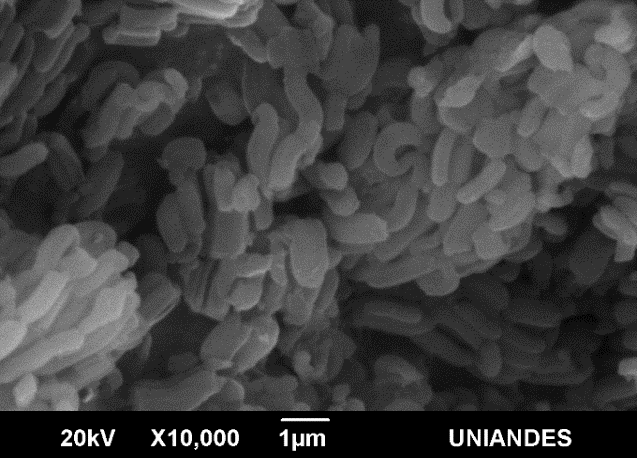
\includegraphics[width=0.9\linewidth]{structures/SEM.png}
	\end{wrapfigure}
	Se llev\'o a cabo la s\'intesis de un material mesoporoso del tipo SBA-15, el cual posteriormente fue funcionalizado con un grupo amino. La preparaci\'on sigue la ruta de Zhao 1998, la cual hace uso del copolimero tribloque Pluronic 123, el cual consiste en una cadena polim\'erica de \'oxido de polietileno, y \'oxido de polipropileno. La funcionalizaci\'on se realiza luego de la obtenci\'on del compuesto mesoporoso, usando una soluci\'on de 3-aminopropiltrietoxisilano en etanol y reflujo por 3 horas. El an\'alisis de resultados se realiza usando informaci\'on proporcionada por el grupo de Calorimetr\'ia y S\'olidos Porosos de la Universidad de los Andes.}

%----------------------------------------------------------------------------------------

\begin{document}

\flushbottom % Makes all text pages the same height

\maketitle % Print the title and abstract box

%\tableofcontents % Print the contents section

\thispagestyle{empty} % Removes page numbering from the first page



%----------------------------------------------------------------------------------------
%	ARTICLE CONTENTS
%----------------------------------------------------------------------------------------

\section*{Introducci\'on} % The \section*{} command stops section numbering

Los materiales mesoporosos son aquellos que presentan poros con tama\~nos entre los 20 \r{A} y 500 \r{A} \cite{macnaught_wilkinson_1997}, los mismos han sido ampliamente estudiados por su demanda en reacciones y separaciones de compuestos de alto peso molecular \cite{zhao_1998}. Los materiales mesoporosos se obtienen a partir de variedad de compuestos, siendo los m\'as comunes aquellos de s\'ilica y al\'umina \cite{mitra_bhaumik_paul_2008}. Existen adem\'as algunos ejemplos de \'oxidos de metales de transici\'on como el niobio, t\'antalo, tit\'anio, y zirconio \cite{lee_lu_kondo_domen_2002}\cite{noda_lee_domen_kondo_2008}\cite{mitra_bhaumik_paul_2008}\cite{parvulescu_bonnemann_parvulescu_endruschat_rufinska_lehmann_tesche_poncelet_2001}.

Las s\'ilicas porosas presentan propiedades importantes como resistencia mec\'anica, \'area superficial y tama\~no del poro uniforme. Los mayores exponentes de los compuestos mesoporosos basados en el silicio son el MCM-41, sintetizado en 1992 por Mobil Corporation con una geometr\'ia unidimensional cil\'indrica \cite{zhao_1998}. Por otro lado la SBA-15 (\textit{tipo de material Amorfo Santa Barbara} del ingl\'es \textit{Santa Barbara Amorphous type material}), sintetizada en 1997 en la Universidad de California en Santa Barbara, es un tipo de material mesoporoso con poros de tama\~nos entre 46 y 300 \r{A} y geometr\'ia bidimencional hexonal \cite{zhao_1998}.

Debido a la escala de las nanopart\'iculas, se han desarrollado una gran variedad de condiciones para explorar el direccionamiento estructural que presentan las interacciones electroest\'aticas, puentes de hidr\'ogeno y van der Waals, en la s\'intesis de compuestos mesoporosos \cite{zhao_1998}. En el caso del MCM-41 y la SBA-15, para el primero se hace uso de surfactantes cati\'onicos, mientras que para la segunda se usan no i\'onicos \cite{zhao_1998}. Para la preparaci\'on de la SBA-15 es posible usar gran variedad de tensoactivos, los cuales le agregan diferentes propiedades al s\'olido obtenido. A pesar que un \'unico surfactante es suficiente, los mejores resultados son obtenidos usando una combinaci\'on de dos tensoactivos conocida como Pluronic 123, el cual consiste en una cadena polim\'erica de tres bloques de copol\'imeros (\autoref{eq: pluronic}): \'oxido de polietileno (EO), \'oxido de polipropileno (PO), y nuevamente \'oxido de polietileno (EO). Los surfactantes anteriores hacen parte de una familia de tensoactivos muy usados en la emulsificaci\'on, solubilizaci\'on, lubricaci\'on, adem\'as de ser usados como espumantes y farmace\'uticos \cite{zhao_1998}.
\begin{equation} \label{eq: pluronic}
    \ce{EO_{20}-PO_{70}-EO_{20}} \qquad \text{Pluronic 123}
\end{equation}

El procedimiento general para la obtenci\'on de compuestos mesoporosos es la formaci\'on de miscelas, la polimerizaci\'on y crecimiento de la red estructural, y posterior calcinaci\'on con el objetivo de eliminar el surfactante y restos de disolvente en la estructura porosa.

En la s\'intesis de la estructura mesoporosa mostrada en el presente documento se hace uso de tetraetil ortosilicato (TEOS) como fuente de silicio para la formaci\'on de la red estructural, Pluronic 123 como surfactante para la formaci\'on de miscelas, y con el objetivo de alcanzar el punto isoel\'ectrico del silicio se usa \'acido clorh\'idrico. Siguiendo la s\'intesis de Zhao \cite{zhao_1998}. Posteriormente se realiza una funcionalizaci\'on de la superficie de la SBA-15 con 3-aminopropiltrietoxisilano (APTES) \cite{vargas_legnoverde_giraldo_basaldella_moreno-pirajan_2010}.

\begin{scheme}[h]
    \centering
    \begin{tabular}{cc}
    	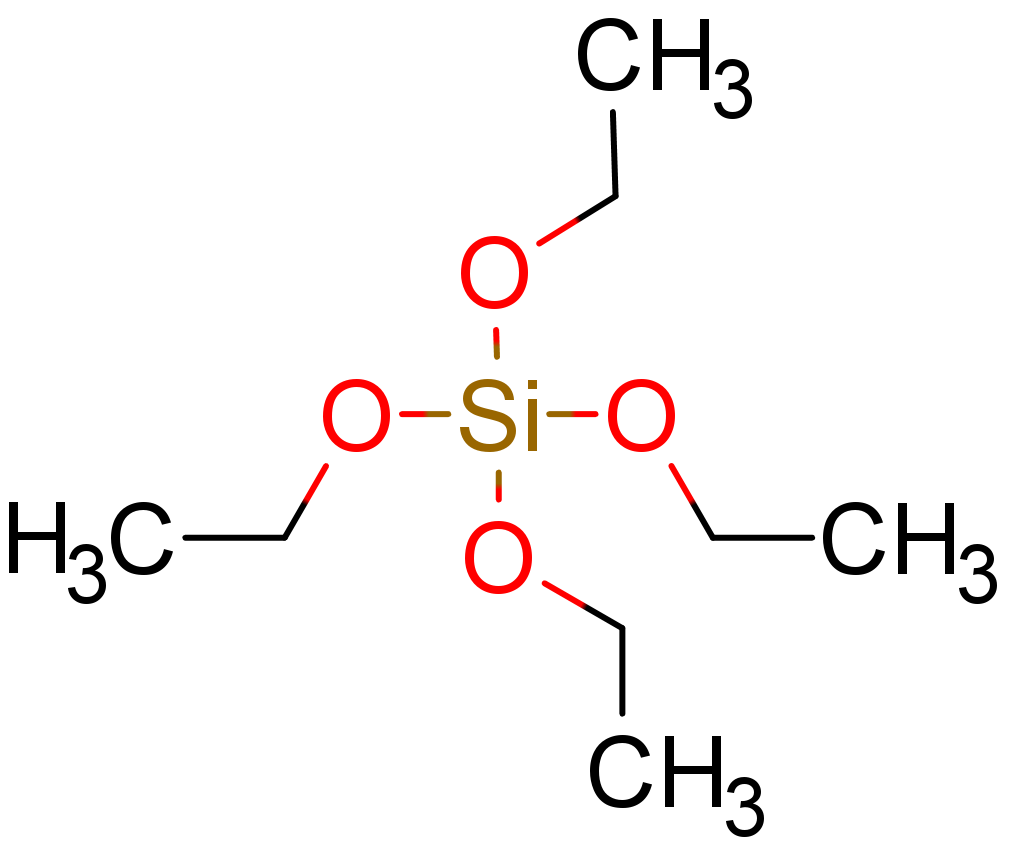
\includegraphics[width=0.3\linewidth]{structures/silicate.png} & 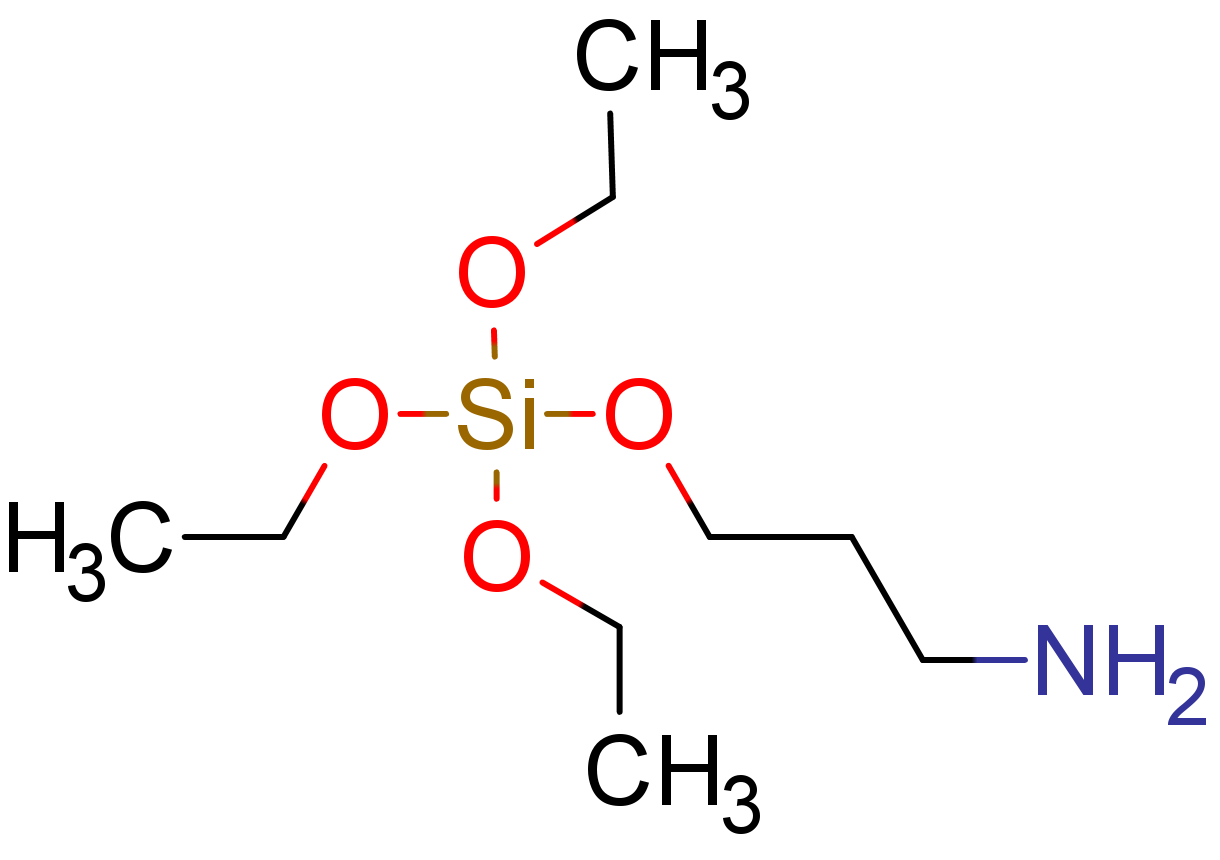
\includegraphics[width=0.4\linewidth]{structures/aminosilicate.png}
    \end{tabular}
	
    \caption{Estructura del tetraetil ortosilicato y 3-aminopropiltrietoxisilano.}
    \label{scheme: sources}
\end{scheme}

\begin{scheme*}[ht]
	\centering
	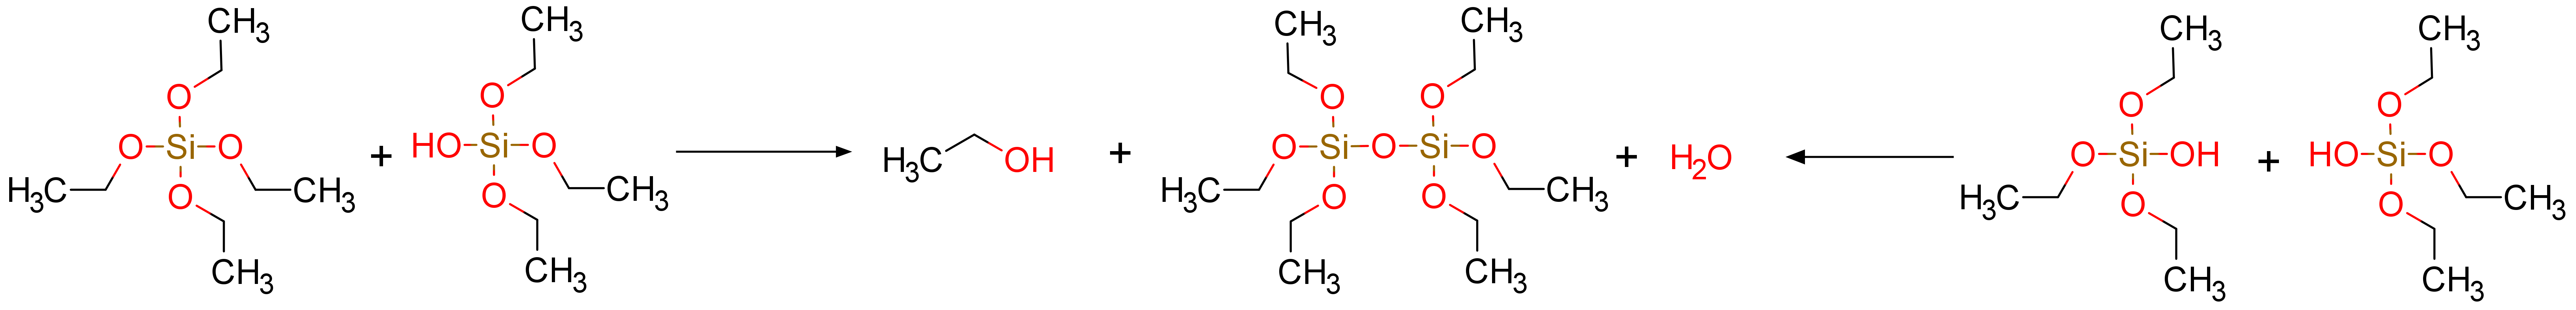
\includegraphics[width=\linewidth]{structures/polysilicate.png}
	\caption{Formaci\'on de una red estructural. De izquierda a derecha la condensaci\'on con salida de etanol, y de derecha a izquierda condensaci\'on de agua.}
	\label{sch: polysilicate}
\end{scheme*}

La caracterizaci\'on de los compuestos mesoporosos incluye gran variedad de t\'ecnicas, entre las que se encuentran: microsc\'opicas, espectrosc\'opicas, adsortivas, termogravim\'etricas y termodin\'amicas. \cite{vargas_legnoverde_giraldo_basaldella_moreno-pirajan_2010}. Las t\'ecnicas de microscop\'ia electr\'onicas son el barrido electr\'onico (SEM) y de transferencia electr\'onica (TEM), la primera se usa con el objetivo de observar la superficie de las nanopart\'iculas y la segunda la estructura interna, que da informaci\'on sobre la porosidad de las mismas. La Fluorescencia de rayos X por energía dispersiva (EDX) permite determinar la relaci\'on nitr\'ogeno silicio en la muestra de SBA-15 funcionalizada con grupos amino, y la resonancia magn\'etica nuclear usando el \'angulo m\'agico para el \ce{^{29}Si}, permite obtener informaci\'on sobre los distintos ambientes qu\'imicos del silicio en la muestra \cite{zhao_1998}. La capacidad de adsorci\'on de un material se cuantifica usando isotermas de adsorci\'on. Los termogramas de una muestra permiten conocer la composici\'on de la misma en funci\'on de la temperatura. Finalmente los an\'alisis termodin\'amicos permiten conocer entalp\'ias, y estados qu\'imicos o f\'isicos de la muestra \cite{vargas_legnoverde_giraldo_basaldella_moreno-pirajan_2010}.

Las isot\'ermas de adsorci\'on se realizan usando nitr\'ogeno gaseoso, para una presi\'on determinada se mide el volumen de nitr\'ogeno obtenido luego de pasar sobre la muestra, dado que se conoce el volumen total introducido es posible calcular el volumen adsorbido por el material. La informaci\'on obtenida se relaciona con la teor\'ia de Brunauer–Emmett–Teller (BET), la cual da cuenta del proceso de adsorci\'on y desorci\'on usando como hip\'otesis: que las mol\'eculas de un gas pueden ser f\'isicamente adsorbidas por una capa de un s\'olido indefinidamente, no existe ninguna interacci\'on entre las capas del s\'olido, y los gases se comportan como gases ideales. La teor\'ia BET permite calcular el \'area superficial de un compuesto mesoporoso.

Finalmente, los compuestos mesoporosos de silicio funcionalizados se encuentran bajo estudio como sistemas de entrega de medicamentos debido a la estabilidad de los poros, la forma de su superficie, adem\'as de ser biocompatibles, entre los cuales los m\'as promisorios presentan grupos aminos \cite{vargas_legnoverde_giraldo_basaldella_moreno-pirajan_2010}.
%------------------------------------------------

\section{Resultados y Discusi\'on}
\begin{figure}[h]
	\centering
	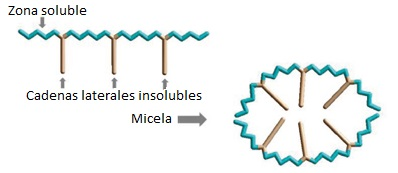
\includegraphics[width=0.8\linewidth]{structures/Micela.jpg}
	\caption{Formaci\'on de micelas por el copol\'imero Pluronic 123. Modificado de \cite{grallert_rangel_yagui_pasqualoto_tavares_2012}.}
	\label{fig: micela}
\end{figure}
El Pluronic 123 tiene a sus extremos dos copol\'imeros solubles, mientras que en el medio se cuentra el polipropileno, el cual presenta una cadena lateral poco polar. Los polietilenglicoles de los extremos forman puentes de hidr\'ogeno con el agua, haciendo de los mismos una parte hidrof\'ilica, las cadenas laterales (metilos) del polipropilenglicol forman la parte hidrof\'obica, dando lugar a la formaci\'on de micelas de la forma ilustrada en la \autoref{fig: micela}.

Por otro lado la disoluci\'on del tetraetil ortosilicato en agua, da lugar a la hidr\'olisis del mismo, siguiendo un mecanismo S$_\text{N2}$ en donde un ox\'igeno del enlace carbono ox\'igeno ataca a un hidr\'ogeno del agua, protonando el ox\'igeno del \'eter de sililo. Posteriormente el \ce{OH-} ataca al carbono en $\alpha$ al ox\'igeno, generando la salida del mismo. 
\begin{scheme}[h]
	\centering
	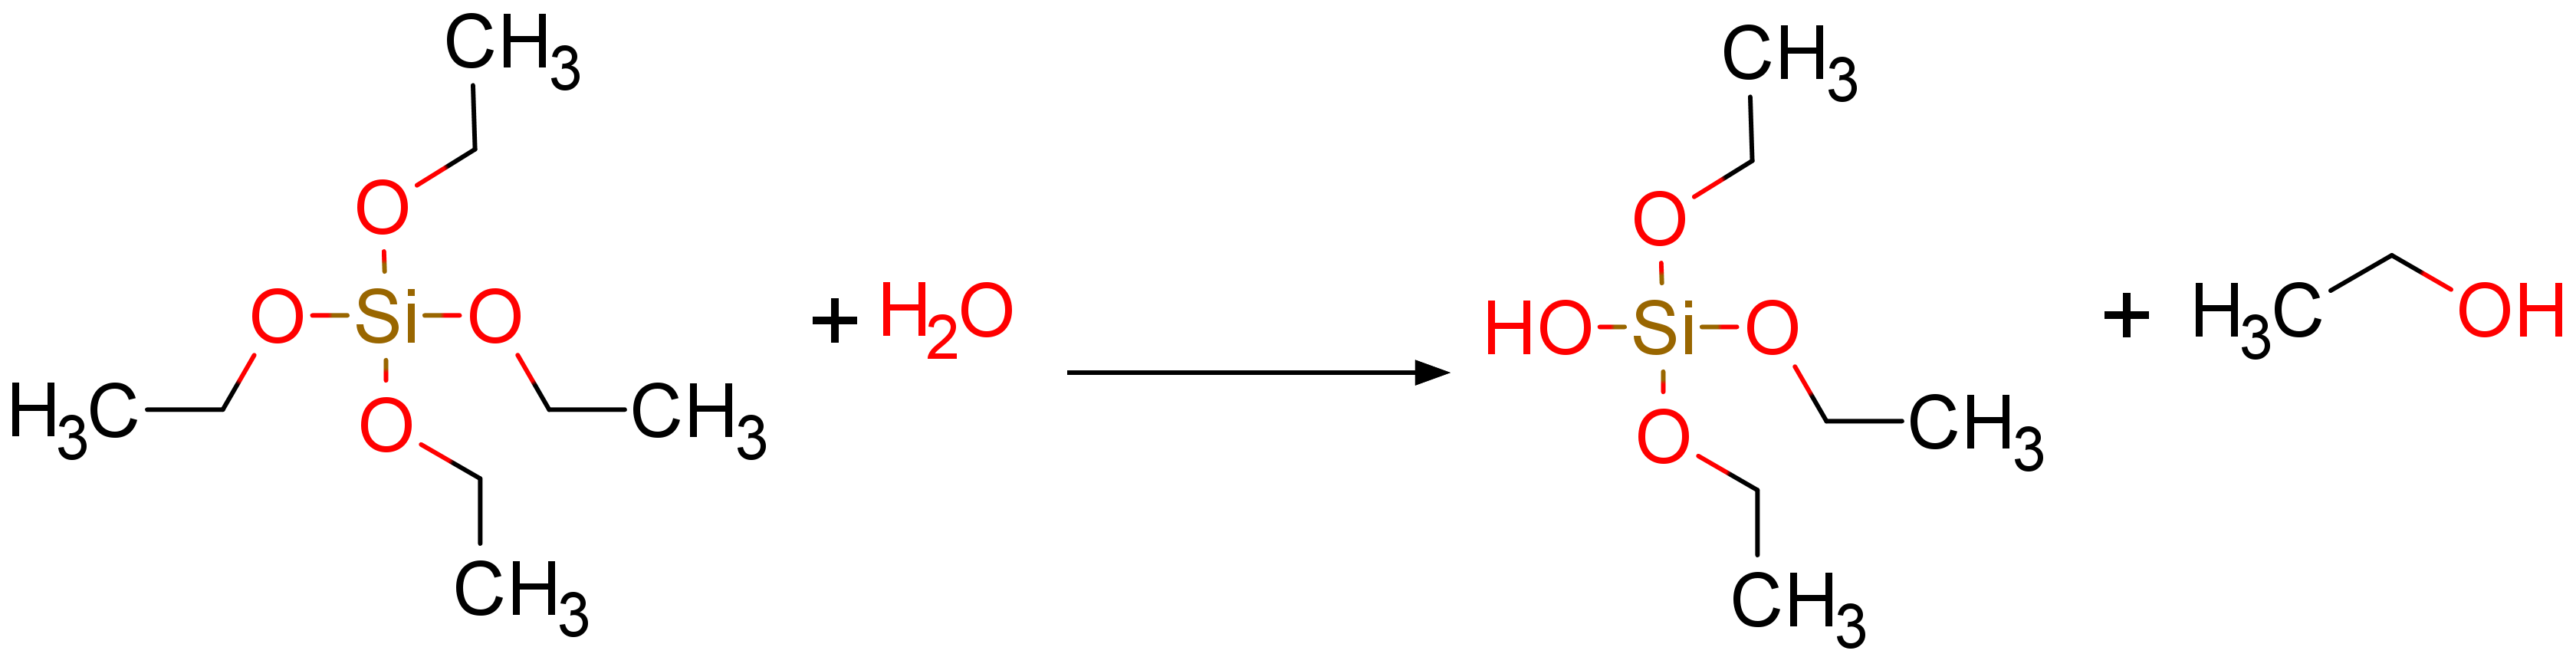
\includegraphics[width=\linewidth]{structures/hidrosilicate.png}
	\caption{Hidr\'olisis del tetraetil ortosilicato en soluci\'on acuosa.}
	\label{sch: hidrosilicate}
\end{scheme}
\begin{scheme}[h]
	\centering
	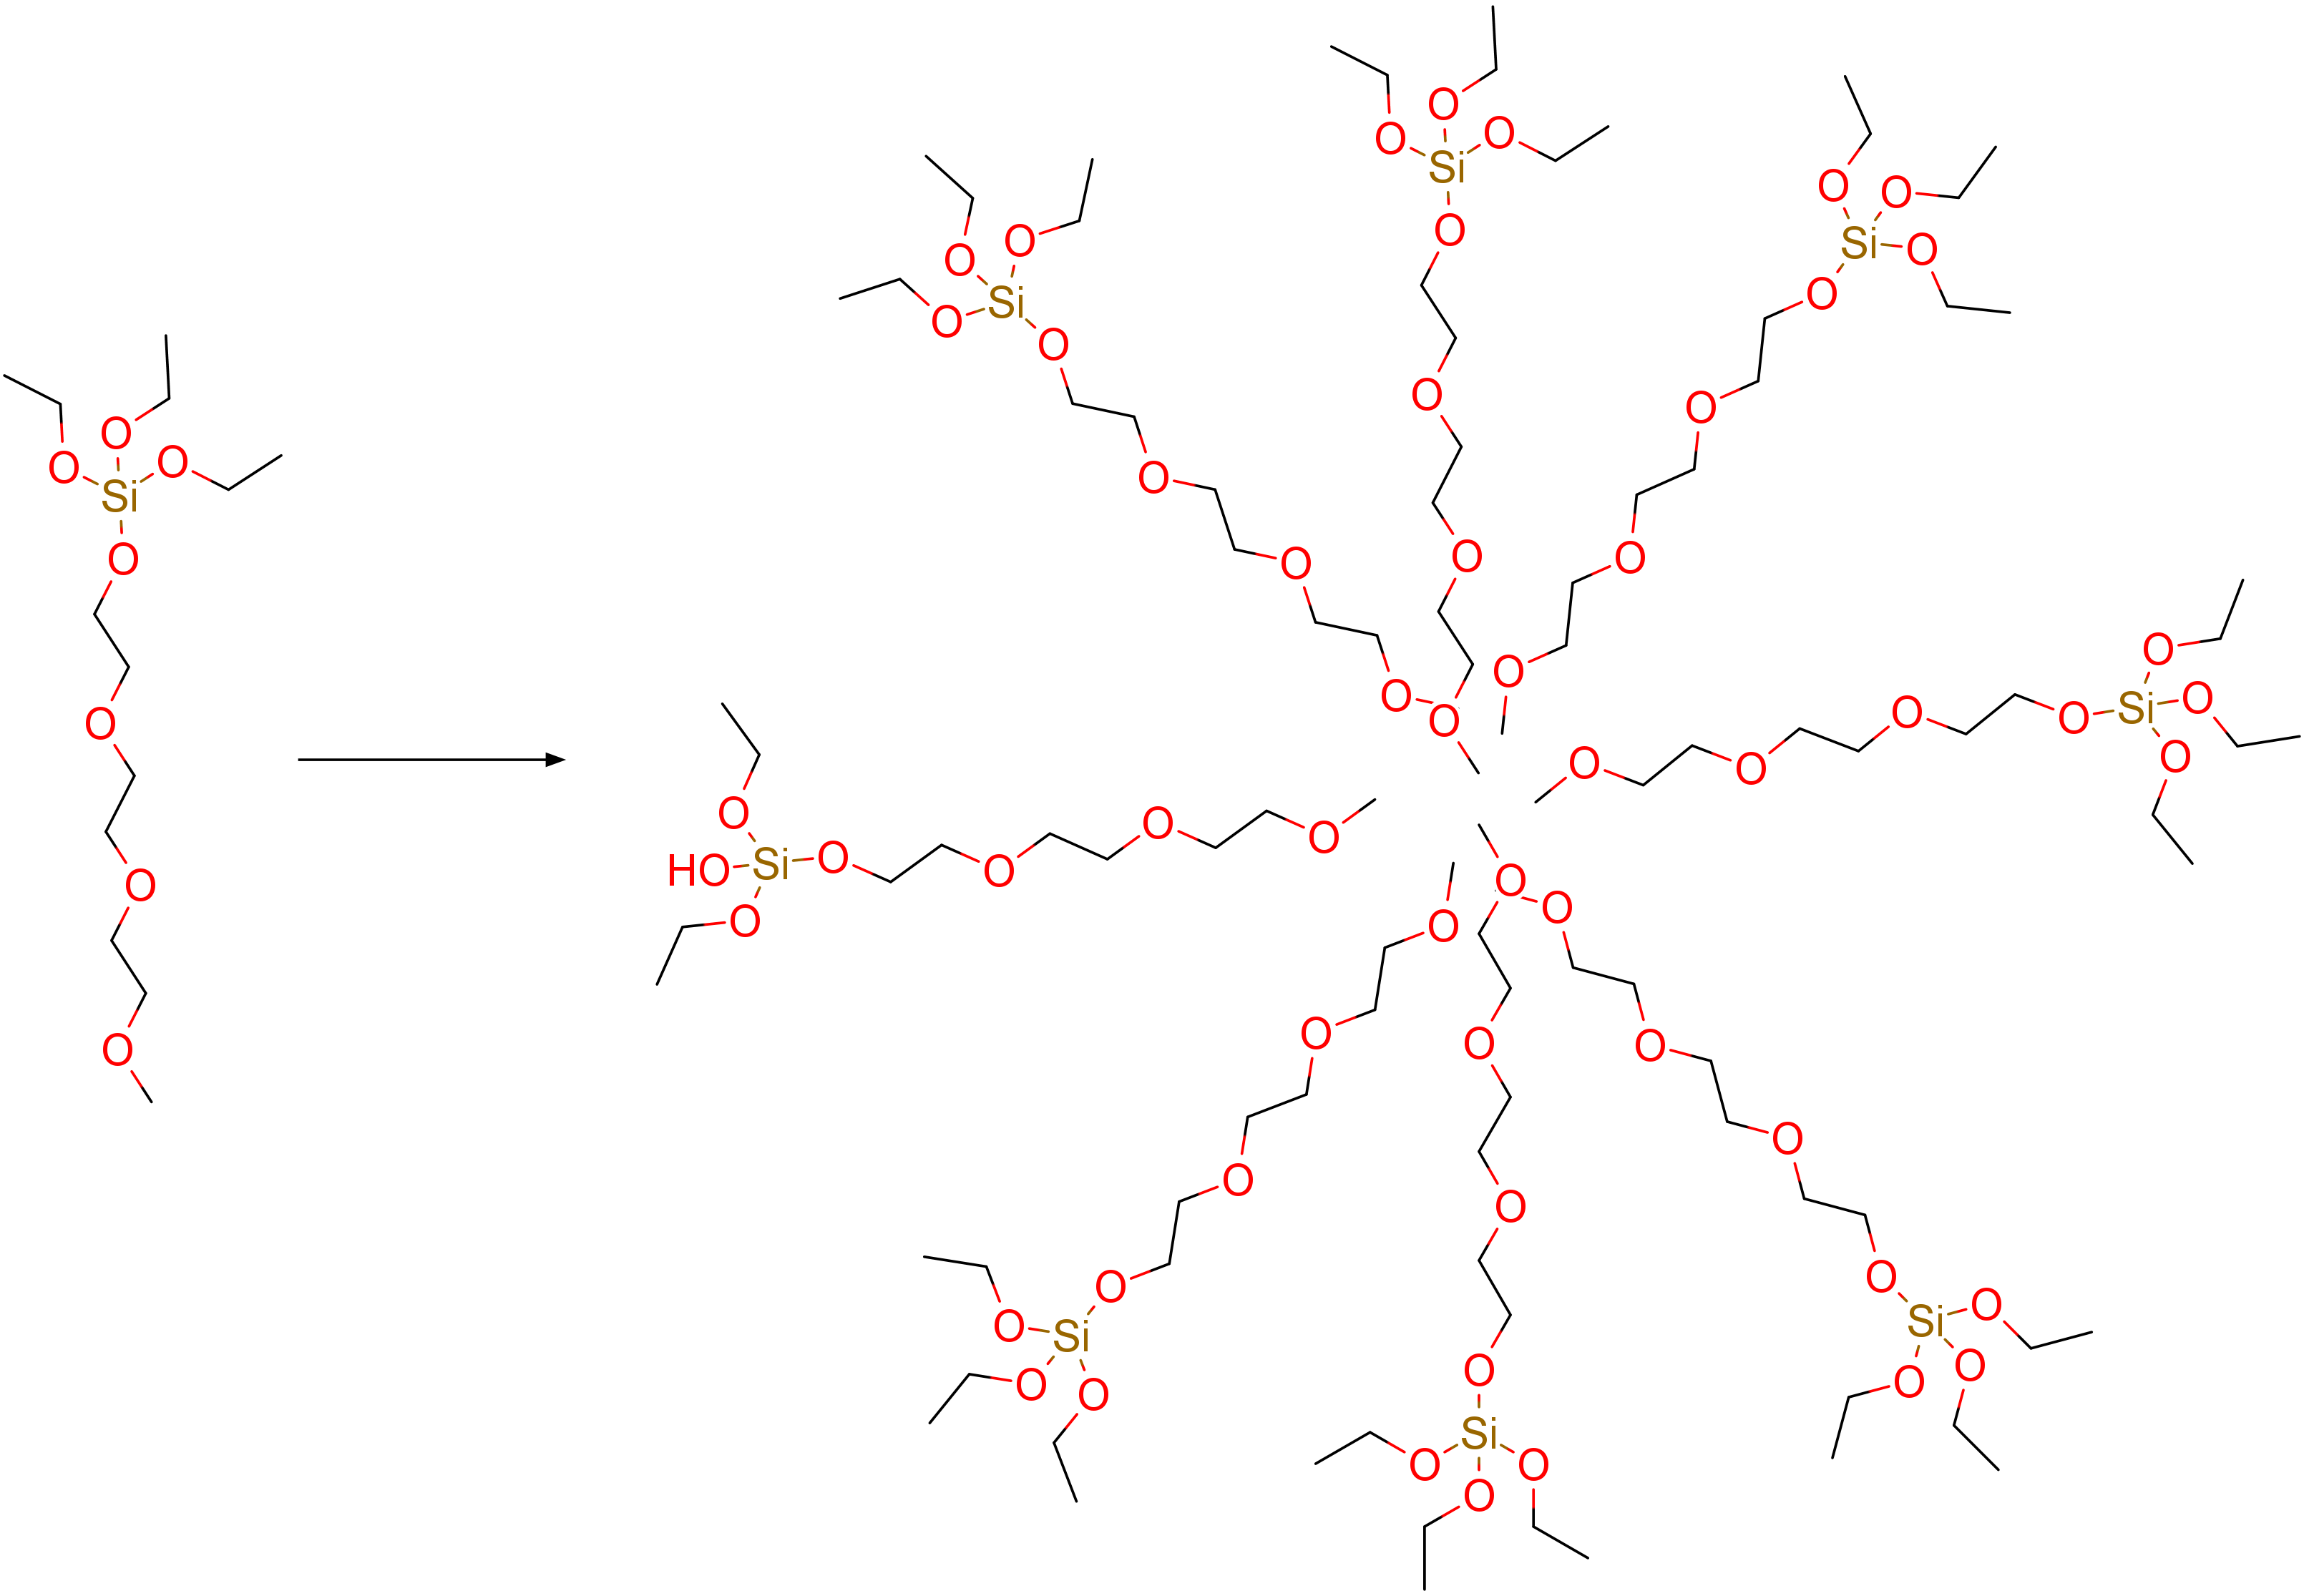
\includegraphics[width=\linewidth]{structures/micelaSi.png}
	\caption{Formaci\'on de las micelas con la incorporaci\'on del silicio \cite{yang_2011}.}
	\label{sch: micelaSi1}
\end{scheme}

El tetraetil ortosilicato hidrolizado puede condensarse con otra mol\'ecula de hidrolizada o el \'eter de sililo normal, dando lugar a la formaci\'on de un enlace silanol como se muestra en el \autoref{sch: polysilicate}. El mismo puede hidrolizarse nuevamente y condensarse, generando la formaci\'on de una red alrededor de la estructura cil\'indrica. Zhao en su publicaci\'on de 1998, sugieren que debe existir un balance entre las interacciones de Coulomb, enlaces de hidr\'ogeno y van der Waals con el objetivo de incrementar la peri\'odicidad a largo rango para la obtenci\'on de estructuras de alto orden. Para esto se lleva la s\'ilica debajo de su punto isoel\'ectrico, generando una especie cationica de la misma. Un mecanismo designado como \ce{(S^0H^+)(X^-I^+)} que incluye las interacciones antes descritas, fue propuesto para explicar la formaci\'on de estructuras mesoporosas de s\'ilica en presencia de surfactantes no ionicos \cite{yang_2011}.
 
Una vez adicionada la fuente de silicio, las micelas modifican su geometr\'ia y hebra a hebra se condensa con el \'eter de sililo, \autoref{sch: micelaSi1}.
\begin{scheme}[h]
	\centering
	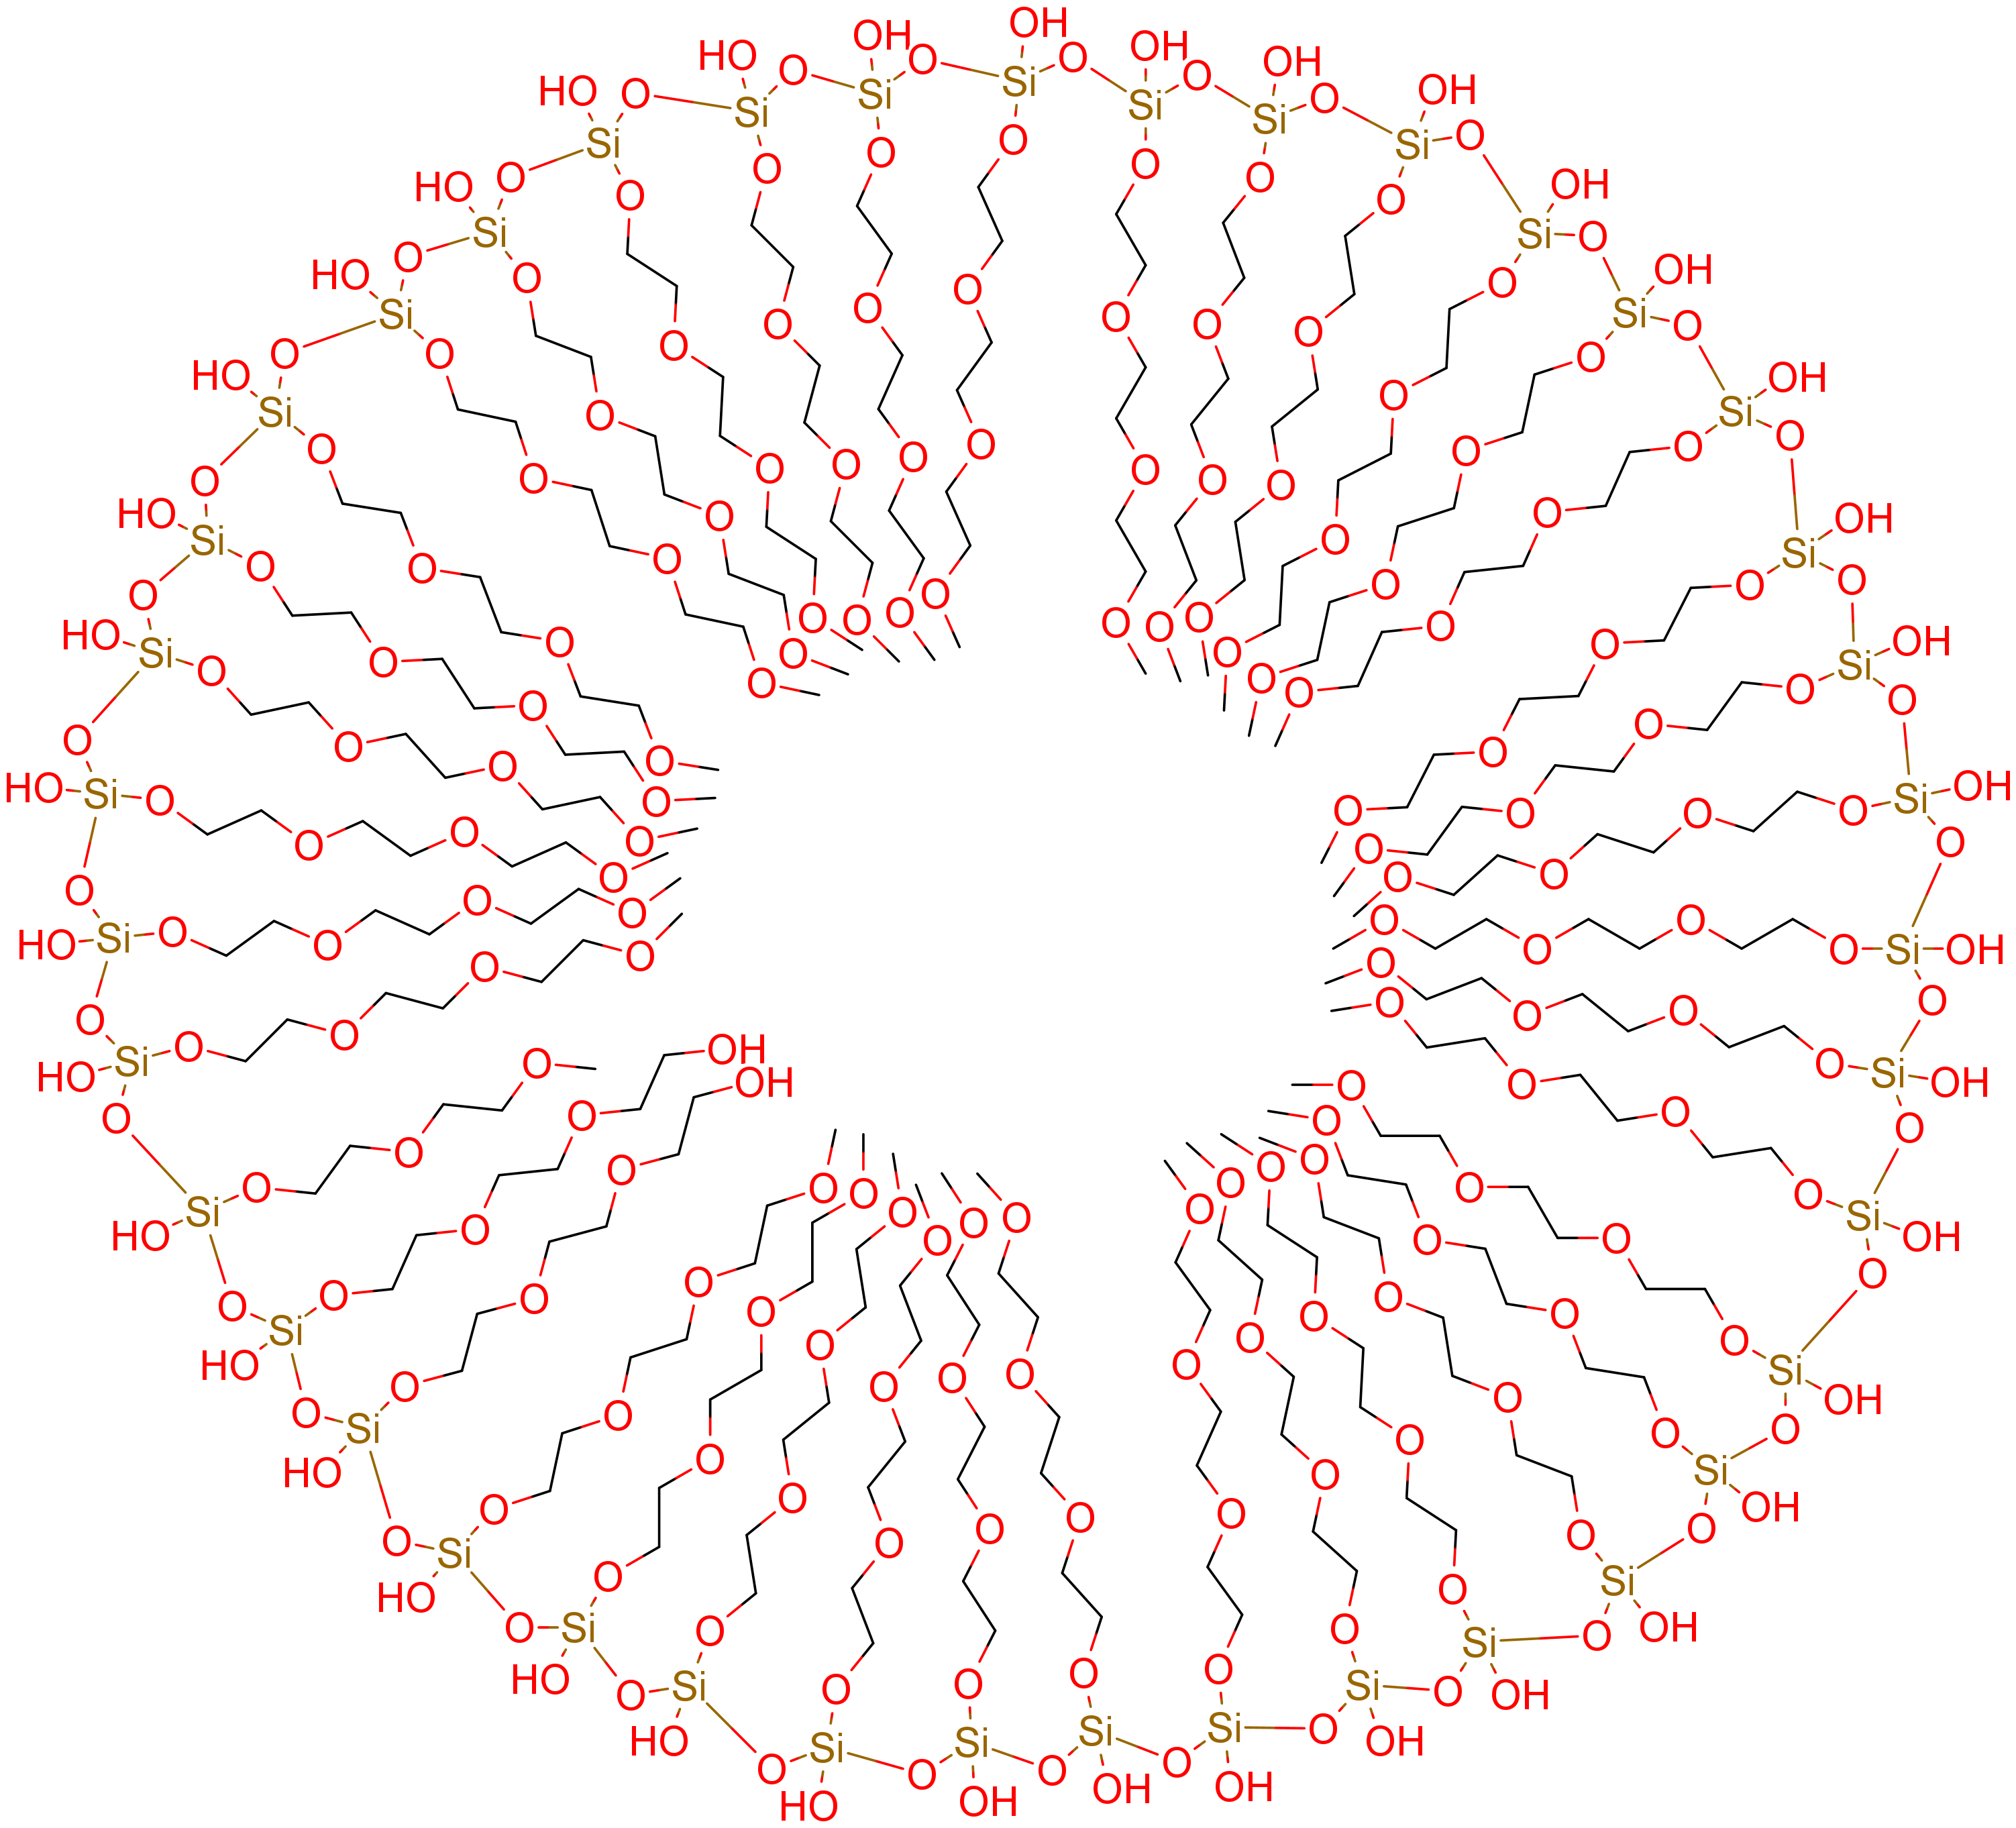
\includegraphics[width=0.8\linewidth]{structures/micelaSi2.png}
	\caption{Formaci\'on de las micelas con la incorporaci\'on del silicio \cite{yang_2011}.}
	\label{sch: micelaSi2}
\end{scheme} 

La formaci\'on de micelas en la soluci\'on constituye la primera etapa en la formaci\'on de los compuestos mesoporos. Las hebras se condensan intermolecularmente entre ellas siguiendo lo mostrado en el \autoref{sch: polysilicate}, formando un caparaz\'on de silanol. Con el hidroxilo restante las micelas tienden a unirse formando una estructura tridimensional cil\'indrica como en la \autoref{fig: micela3d}. Incrementando el aislamiento de los grupos m\'as hidrof\'obicos al interior del cil\'indro.
\begin{figure}[h]
	\centering
	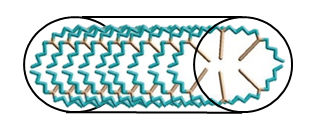
\includegraphics[width=0.8\linewidth]{structures/micela3D.png}
	\caption{Formaci\'on de estructuras cil\'indricas por parte de las micelas.}
	\label{fig: micela3d}
\end{figure}

Los cilindros se agupan en grupos de seis dando lugar a la formaci\'on de estructuras hexagonales. Finalmente con el proceso de calcinaci\'on se elimina el contenido interno de las estructuras con la descomposici\'on del copolimero que se encuentra en el mismo, dado que la temperatura de descomposici\'on es cercana a 150 $^\circ$C ligada a la SBA-15 y 250 $^\circ$C cuando se encuentra pura \cite{zhao_1998}. Lo anterior se puede observar en el an\'alisis termogravim\'etrico de una muestra de SBA-15 sintetizada por el grupo de Calorimetr\'ia y S\'olidos Porosos en el 2016, en donde se observa una p\'erdida de un 45.5 \% en la masa respecto a la inicial, y el mayor cambio en la regi\'on entre 100 y 300 grados celsius, usando la derivada termogravim\'etrica DTG.
\begin{figure}[h]
	\centering
	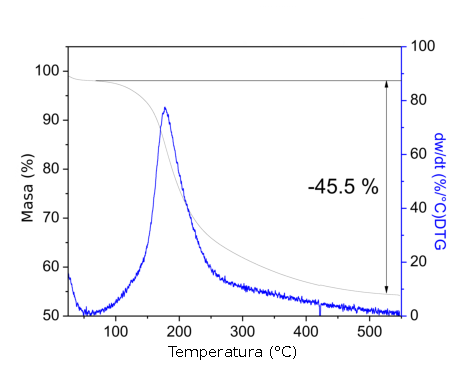
\includegraphics[width=\linewidth]{structures/TGA-calcination.pdf}
	\caption{TGA de la eliminaci\'on del copol\'imero \cite{melendez_murillo_ramirez_2016}.}
	\label{fig: TGA-calcination}
\end{figure}
\pagebreak

Los resultados obtenidos por el microscopio electr\'onico de barrido se muestran en la \autoref{fig: SEM}, en ella se evidencian dominios cil\'indricos con tama\~nos cercanos a 1 $\mu$m, uniformes, los cuales se agrupan en escalas mucho mayores (100 $\mu$m) en estructuras tipo trigo, los cuales son t\'ipicos para la SBA-15 \cite{zhao_1998}\cite{melendez_murillo_ramirez_2016}.
\begin{figure}[h]
    \centering
    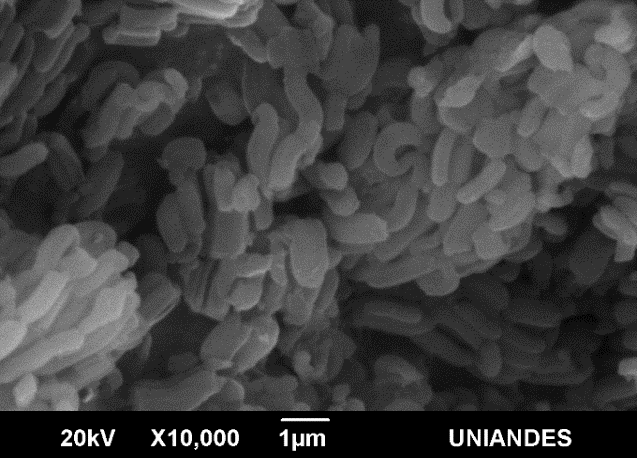
\includegraphics[width=0.8\linewidth]{structures/SEM.png}
    \caption{Imagen de la SBA-15 bajo el microscopio electr\'onico de barrido \cite{melendez_murillo_ramirez_2016}.}
    \label{fig: SEM}
\end{figure}

Las im\'agenes de microscopio electr\'onico de transmisi\'on obtenidas por varios autores, muestran la estructura hexagonal de la misma tanto en la vista lateral como superior \cite{zhao_1998}\cite{vargas_legnoverde_giraldo_basaldella_moreno-pirajan_2010}\cite{zhao_huo_feng_chmelka_stucky_1998}, a partir de la misma los autores reportan tama\~nos de poro entre 47 y 89 \r{A}, y anchos de pared de 31 a 53 \r{A}.
\begin{figure}[h]
    \centering
    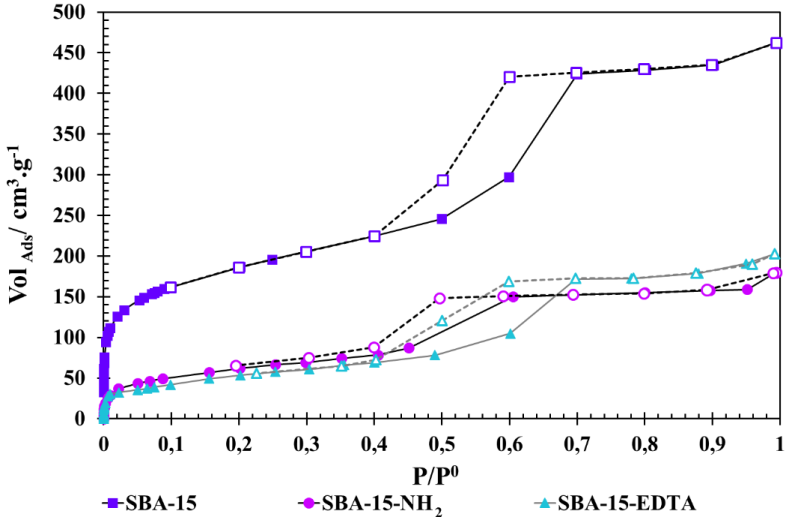
\includegraphics[width=0.8\linewidth]{structures/isotherm.png}
    \caption{Isot\'erma de adsorci\'on y desorci\'on de nitr\'ogeno a $T = -196$ $^\circ$C. Para SBA-15 y dos muestras funcionalizadas con grupos amino y EDTA \cite{rodriguez}.}
    \label{fig: isoterma}
\end{figure}
\begin{figure*}[ht]
	\centering
	\begin{subfigure}[b]{0.45\textwidth}
		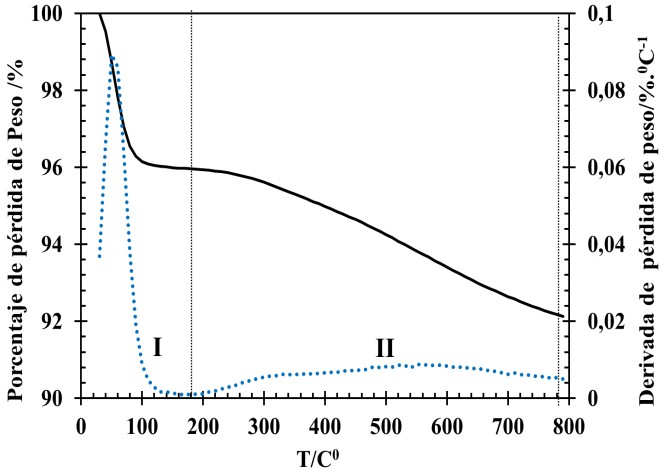
\includegraphics[width=\linewidth]{structures/TGA-normal.png}
		\caption{SBA-15}
		\label{fig: TGA-normal}
	\end{subfigure}
	\begin{subfigure}[b]{0.45\textwidth}
		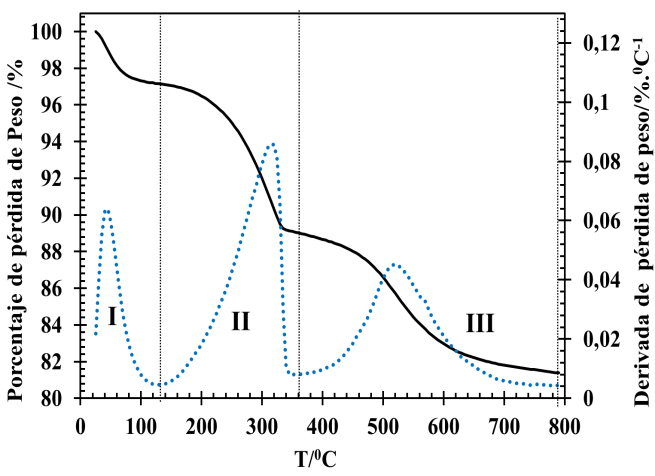
\includegraphics[width=\linewidth]{structures/TGA-NH2.png}
		\caption{SBA-15-\ce{NH2}}
		\label{fig: TGA-NH2}
	\end{subfigure}    
	\caption{Termogr\'amas para compuestos mesoporosos SBA \cite{rodriguez}.}
\end{figure*}

Respecto a las isot\'ermas de adsorci\'on y desorci\'on se observan tres regiones: la absorci\'on de una monocapa y una multicapa, la condensaci\'on capilar y la absorci\'on en la superficie exterior de las part\'iculas \autoref{fig: isoterma}, los cuales corresponden con una curva caracter\'istica de compuestos mesoporosos, tipo IV \cite{vargas_legnoverde_giraldo_basaldella_moreno-pirajan_2010}. Las curvas de adsorci\'on se encuentran clasificadas por la IUPAC, seg\'un la forma de las mismas. Tipo I cuando solo existe adsorci\'on por monocapa, tipo II cuando se observa una zona plano en la curva an\'aloga a una funci\'on polin\'omica de grado 3, donde la regi\'on en particular se debe a la formaci\'on de la monocapa. Tipo III cuando se observa adsorci\'on por multicapa, y las curvas tipo IV presentan todas las anteriores, en donde el nivel de saturaci\'on se alcanza a una presi\'on menor a la presi\'on de vapor, lo anterior se explica con la condensaci\'on de gas en  regiones capilares de los mesoporos \cite{sing_2001}. En el caso de la funcionalizaci\'on con grupos amino, se observa una disminuci\'on en el tama\~no del poro, lo cual es evidencia de el anclaje de las mol\'eculas de APTES a la superficie \cite{vargas_legnoverde_giraldo_basaldella_moreno-pirajan_2010}.

La modificaci\'on a la SBA consiste en una reacci\'on qu\'imica entre los grupos hidroxi del s\'olido y el \'eter de sililo con el grupo de inter\'es. Debido a la calcinaci\'on de la muestra, los ox\'igenos disponibles se encuentran en el interior de los poros, por lo cual los grupos funcionales a introducir estar\'an preferiblemente en estas posiciones. La disminuci\'on en el tama\~no del poro observada en la \autoref{fig: isoterma}, se puede atribuir a que muchas de las mol\'eculas de APTES reaccionan en la parte exterior del poro, dificultando el ingreso de otras al interior del s\'olido, de la misma forma el aumento de las interacciones en la parte exterior del s\'olido dificultan el ingreso de \ce{N2} disminuyendo la capacidad de adsorci\'on del s\'olido. Sin embargo, a\'un cuando se pierde \'area superficial y capacidad de retenci\'on de sustancias, investigadores han determinado experimentalmente que la SBA-15 funcionalizada con grupos aminos presenta a mayor capacidad de retenci\'on de Cefalexina, un antibi\'otico al que se le busca mejorar su transporte en el organismo \cite{vargas_legnoverde_giraldo_basaldella_moreno-pirajan_2010}.

Luego de haber realizado la calcinaci\'on de las muestras un segundo an\'alisis termogravimetrico muestra dos cambios de pendientes importantes para la SBA-15 y tres para la funcionalizada \cite{rodriguez}. Para ambos la primera regi\'on corresponde con temperaturas hasta los 120 $^\circ$C, por lo cual es posible que la p\'erdida de masa se deba a solventes org\'anicos y agua en la muestra, que fueron adsorbidos por el s\'olido por la presencia de los mismos en la atm\'osfera del laboratorio. La segunda regi\'on se relaciona con la degradaci\'on de los copol\'imeros en la muestra. En la misma regi\'on en el s\'olido funcionalizado presenta un refuerzamiento en la p\'erdida de masa por los residuos de APTES no ancladas, cuyo punto de ebullici\'on es de 217 $^\circ$C \cite{hawley_1981}.

El an\'alisis infrarrojo llevado a cabo sobre las muestras de SBA por Paola Rodr\'iguez muestra un claro descenso en la transmitancia a 960 cm$^{-1}$ el cual se atribuye a vibraciones de los grupos silanol, los cuales son m\'as abundantes en el s\'olido puro, respecto al funcionalizado. Adicionalmente en el caso de la SBA con grupos amino se observa una vibraci\'on en 1600 cm$^{-1}$, el cual se atribuye al enlace \ce{N-H} \cite{rodriguez}\cite{li_guo_shi_2010}\cite{melendez_murillo_ramirez_2016}.
\begin{figure}[h]
	\centering
	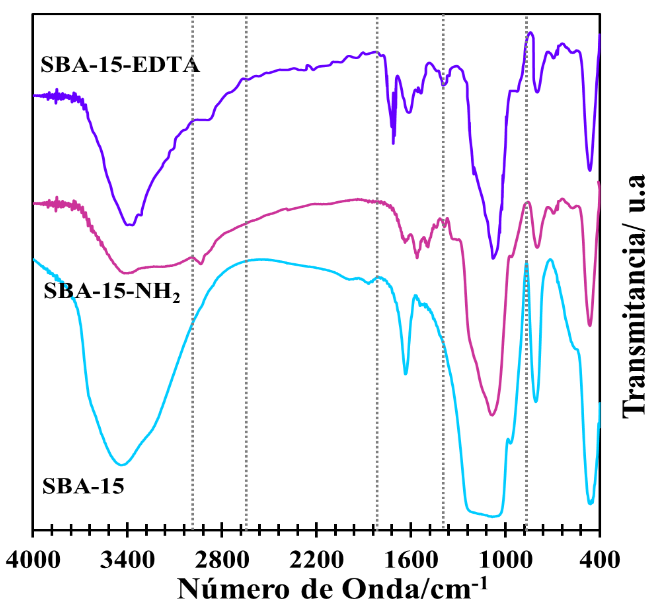
\includegraphics[width=0.8\linewidth]{structures/IR.png}
	\caption{Espectro infrarrojo de distintas muestras de SBA \cite{rodriguez}.}
\end{figure}

\section{Conclusiones}
La s\'intesis del compuesto mesoporoso se llev\'o a cabo siguiendo el procedimiento de Zhao, con el cual fue posible aislar un s\'olido blanco y muy fino \cite{zhao_1998}. A pesar de no ser posible la caracterizaci\'on del mismo, se realiz\'o un estudio con base en productos previos del grupo de investigaci\'on donde tuvo lugar el presente proyecto.
 
La funcionalizaci\'on del s\'olido se llev\'o a cabo usando el procedimiento descrito por Diana Vargas y colaboradores \cite{vargas_legnoverde_giraldo_basaldella_moreno-pirajan_2010}, con lo cual se obtuvo un s\'olido con caracter\'isticas f\'isicas an\'alogas a las descritas para el compuesto mesoporoso normal.
\section{Secci\'on experimental}
La SBA-15 fue preparada siguiendo el procedimiento de Zhao, usando 18.0191 g de Pluronic 123, los cuales fueron disueltos en 135 mL de agua y mantenido bajo agitaci\'on por 3 horas. Una soluci\'on acuosa 2 M de HCl se obtuvo agregando 72 mL de HCl concentrado en 450 mL de agua destilada. Posteriormente y usando un reactor de vidrio y un ba\~no termostatado a 35 $^\circ$C se mezclaron las soluciones previamente descritas, y se agregaron por goteo 42 mL de tetraetil ortosilicato. La mezcla se dej\'o en agitaci\'on por 24 horas, pasados estos se aument\'o la temperatura del reactor a 80 $^\circ$C por otras 24 horas. El s\'olido obtenido fue lavado varias decenas de veces usando agua destilada y filtraci\'on al vac\'io, con el objetivo de eliminar la mayor cantidad de \'acido clorh\'idrico y surfactante. Posteriormente el s\'olido fue calcinado en mufla a una temperatura de 540 $^\circ$C por 6 horas.

La funcionalizaci\'on se lleva acabo usando 2.0412 g de SBA-15 y 6.4 mL de APTES, en 132 mL de etanol absoluto, los cuales se llevan a reflujo por 3 horas, pasado este tiempo se filtra por gravedad y se realizan 3 lavados con etanol. Posteriormente se seca el producto en horno a 80 $^\circ$C.
%----------------------------------------------------------------------------------------
%	REFERENCE LIST
%----------------------------------------------------------------------------------------
\phantomsection
\bibliography{Mesoporosos}
\bibliographystyle{unsrt}

%----------------------------------------------------------------------------------------
\end{document}
